Afin de comparer les performances de RenamableLogootSplit et de LogootSplit de manière globale, nous avons mesuré le temps nécessaire pour un nouveau noeud pour rejouer l'entièreté du log d'opérations d'une session de collaboration, en fonction du nombre de \emph{renaming bots} de la session.
Nous présentons les résultats obtenus dans la \autoref{fig:time-to-replay-log}.

\begin{figure}[!ht]
  \centering
  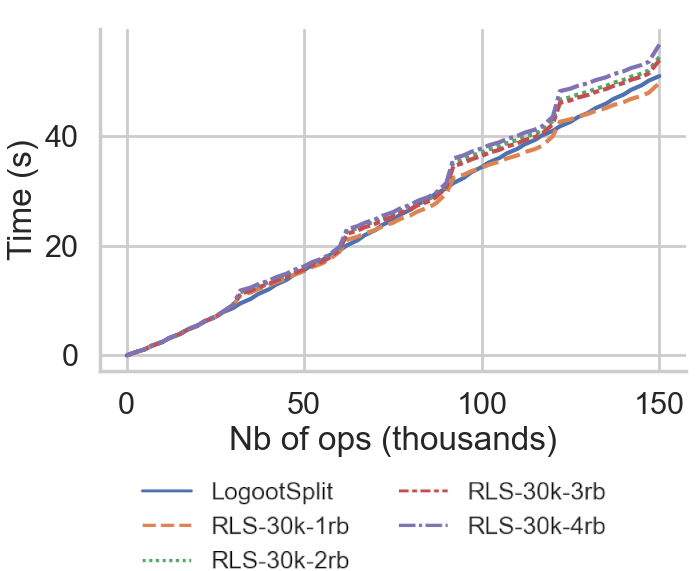
\includegraphics[width=0.7\columnwidth]{img/replay-log-30k-with-legend.png}
  \caption{Progression du nombre d'opérations du log rejouées en fonction du temps}
  \label{fig:time-to-replay-log}
\end{figure}

Nous observons que le gain sur le temps d'intégration des opérations \emph{insert} et \emph{remove} permet initialement de contrebalancer le surcoût des opérations \emph{rename}.
Mais au fur et à mesure que la collaboration progresse, le temps nécessaire pour intégrer les opérations \emph{rename} augmente car plus d'éléments sont impliqués.
Cette tendance est accentuée dans les scénarios avec des opérations \emph{rename} concurrentes.

Dans un cas réel d'utilisation, ce scénario (\ie rejouer l'entièreté du log) ne correspond pas au scénario principal et peut être mitigé, par exemple en utilisant un mécanisme de compression du log d'opérations.
Dans la \autoref{sec:rename-as-compression-mechanism}, nous présentons comment mettre en place un tel mécanisme en se basant justement sur les possibilités offertes par l'opération \emph{rename}.
